\documentclass[a4paper,12pt]{article}
\usepackage[utf8]{inputenc}
\usepackage[spanish]{babel}
\usepackage{amsmath}
\usepackage{amssymb}
\usepackage{amsthm}
\usepackage{geometry}
\usepackage{fancyhdr}
\usepackage{tcolorbox}
\usepackage{booktabs}
\usepackage{multicol}
\usepackage{float}
\usepackage{graphicx}
\usepackage{wrapfig}

\geometry{top=2.5cm, bottom=2.5cm, left=3cm, right=3cm}

% Configuración de encabezado
\setlength{\headheight}{14.49998pt}
\pagestyle{fancy}
\fancyhf{}
\lhead{Licenciatura en Sistemas de Información}
\rhead{Unidad 2: FVV}
\cfoot{\thepage}

\title{\textbf{Resumen Unidad 2: Funciones de Varias Variables}}
\author{Ecuaciones Diferenciales y Cálculo Multivariado}
\date{}

\begin{document}

\maketitle

\part{Topología y Conceptos Básicos}

\section{Conjuntos Puntuales en el Plano y el Espacio}

\subsection{Distancia y Entornos}
En un espacio numérico de $n$ dimensiones, la distancia entre dos puntos está dada por $d = \sqrt{\sum_{i=1}^{n}(x'_{i} - x_i)^2}$.
A partir de este concepto se definen los entornos:
\begin{itemize}

    \noindent
    \begin{minipage}{0.55\textwidth}
        \item \textbf{Disco abierto:} Es el conjunto de puntos del plano con centro en $C(x_0, y_0)$ y radio $r$ que verifica $(x - x_0)^2 + (y - y_0)^2 < r^2$.
    \end{minipage}
    \hfill 
    \begin{minipage}{0.40\textwidth}
        \centering
        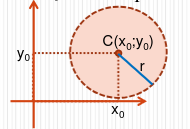
\includegraphics[width=\textwidth]{discoabierto.png} 
    \end{minipage}
       

    \noindent
    \begin{minipage}{0.55\textwidth}
        \item \textbf{Disco cerrado:} Es el conjunto de puntos del plano con centro en $C(x_0, y_0)$ y radio $r$ que verifica $(x - x_0)^2 + (y - y_0)^2 \leqslant r^2$.
    \end{minipage}
    \hfill 
    \begin{minipage}{0.40\textwidth}
        \centering
        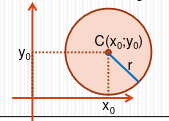
\includegraphics[width=\textwidth]{discocerrado.png} 
    \end{minipage}

    \noindent
    \begin{minipage}{0.55\textwidth}
        \item \textbf{Entorno circular:} Es el conjunto de puntos del plano con centro en $C(x_0, y_0)$ y radio $r$ que verifica $(x - x_0)^2 + (y - y_0)^2 < r^2$. Simbólicamente se denota $E(C, r)$.
    \end{minipage}
    \hfill 
    \begin{minipage}{0.40\textwidth}
        \centering
        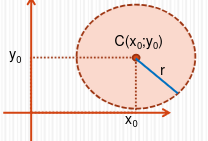
\includegraphics[width=\textwidth]{entornocircular.png} 
    \end{minipage}

    \noindent
    \begin{minipage}{0.55\textwidth}
        \item \textbf{Entorno circular reducido:} Excluye el centro $C$. Se denota $E'(C, r)$ y verifica $0 < (x - x_0)^2 + (y - y_0)^2 < r^2$.
    \end{minipage}
    \hfill 
    \begin{minipage}{0.40\textwidth}
        \centering
        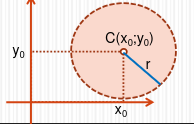
\includegraphics[width=\textwidth]{entornocircularreducido.png} 
    \end{minipage}

    \noindent
    \begin{minipage}{0.55\textwidth}
    \item \textbf{Intervalo rectagular abierto:} es el conjunto de puntos del plano que verifican $a < x < b \land c < y < d$.
    \end{minipage}
    \hfill 
    \begin{minipage}{0.40\textwidth}
        \centering
        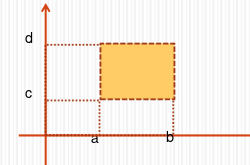
\includegraphics[width=\textwidth]{intervalorectangularabierto.png} 
    \end{minipage}

    \noindent
    \begin{minipage}{0.55\textwidth}
    \item \textbf{Intervalo rectagular cerrado:} es el conjunto de puntos del plano que verifican $a \leq x \leq b \land c \leq y \leq d$.
    \end{minipage}
    \hfill 
    \begin{minipage}{0.40\textwidth}
        \centering
        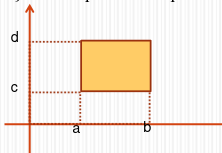
\includegraphics[width=\textwidth]{intervalorectangularcerrado.png} 
    \end{minipage}

    \noindent
    \begin{minipage}{0.55\textwidth}
    \item \textbf{Entorno rectangular:} Con centro en $C$ y semi-amplitudes $d$, verifica $|x - x_0| < d \land |y - y_0| < d$.
    \end{minipage}
    \hfill 
    \begin{minipage}{0.40\textwidth}
        \centering
        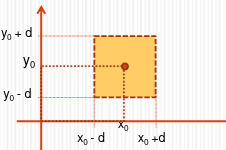
\includegraphics[width=\textwidth]{entornorectangular.png} 
    \end{minipage}

    \noindent
    \begin{minipage}{0.55\textwidth}
    \item \textbf{Entorno rectangular reducido:} Con centro $C$. Verifica $0 < |x - x_0| < d \land 0 < |y - y_0| < d$.
    \end{minipage}
    \hfill 
    \begin{minipage}{0.40\textwidth}
        \centering
        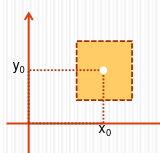
\includegraphics[width=\textwidth]{entornorectangularreducido.png} 
    \end{minipage}

\end{itemize}

\subsection{Clasificación de Puntos}
Dado un conjunto de puntos $S \subseteq \mathbb{R}^2$:
\begin{itemize}
    \item \textbf{Punto interior:} Existe al menos un entorno del punto totalmente contenido en $S$.
    \item \textbf{Punto exterior:} Existe un entorno del punto que no contiene ningún elemento de $S$.
    \item \textbf{Punto frontera:} Todo entorno del punto contiene elementos que pertenecen a $S$ y elementos que no pertenecen a $S$.
    \item \textbf{Punto de acumulación:} En todo entorno reducido del punto hay al menos un elemento que pertenece a $S$.
    \item \textbf{Punto aislado:} Existe un entorno del punto que no contiene otros puntos del conjunto $S$.
\end{itemize}

\subsection{Partes del conjunto}
\begin{itemize}
    \item \textbf{Interior ($\overset{\circ}{S}$):} Conjunto de puntos interiores de $S$.
    \item \textbf{Frontera ($\partial S$):} Conjunto de puntos frontera de $S$.
    \item \textbf{Exterior ($S^c$):} Conjunto de puntos exteriores a $S$.
\end{itemize}

\subsection{Clasificación de Conjuntos}
\begin{itemize}
    \noindent
    \begin{minipage}{0.55\textwidth}
        \item \textbf{Acotado:} Existe un número $k \in \mathbb{R}, k > 0 / \forall (x,y) \in S$ se encuentra dentro de un entorno de radio $k$.
    \end{minipage}
    \hfill 
    \begin{minipage}{0.40\textwidth}
        \centering
        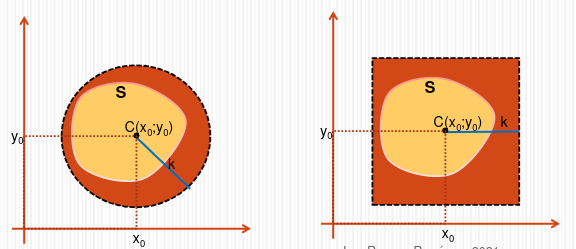
\includegraphics[width=\textwidth]{conjuntoacotado.png} 
    \end{minipage}

    \noindent
    \begin{minipage}{0.55\textwidth}
        \item \textbf{Conexo:} Dos puntos cualesquiera del conjunto se pueden unir por una poligonal contenida enteramente en el conjunto.
    \end{minipage}
    \hfill 
    \begin{minipage}{0.40\textwidth}
        \centering
        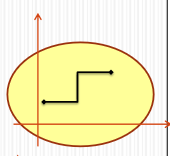
\includegraphics[width=\textwidth]{conjuntoconexo.png} 
    \end{minipage}

    \noindent
    \begin{minipage}{0.55\textwidth}
        \item \textbf{Simplemente conexo:} Es un conjunto conexo donde toda región interior a una poligonal cerrada pertenece al conjunto (no tiene "agujeros").
    \end{minipage}
    \hfill 
    \begin{minipage}{0.40\textwidth}
        \centering
        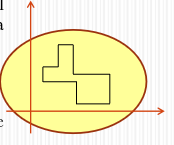
\includegraphics[width=\textwidth]{conjuntosimplementeconexo.png} 
    \end{minipage}

    \noindent
    \begin{minipage}{0.55\textwidth}
        \item \textbf{Múltiplemente conexo:} Es un conjunto conexo que no es simplemente conexo que en su interior tiene "agujeros" (puntos que no pertenecen al conjunto).
    \end{minipage}
    \hfill 
    \begin{minipage}{0.40\textwidth}
        \centering
        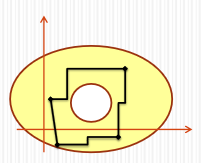
\includegraphics[width=\textwidth]{conjuntomultiplementeconexo.png} 
    \end{minipage}
    
    \item \textbf{Región:} Reunión de un conjunto conexo abierto con algunos, todos o ninguno de sus puntos frontera.
    \item \textbf{Región cerrada:} Si la región contiene todos sus puntos frontera.
    \item \textbf{Región abierta:} Si la región contiene solo sus puntos interiores.
\end{itemize}

\section{Funciones de Varias Variables}

\subsection{Definición, Dominio e Imagen}

    \noindent
    \begin{minipage}{0.55\textwidth}
        Una función de dos variables $z = f(x,y)$ asigna a cada par ordenado $(x,y) \in D \subseteq \mathbb{R}^2$ un único número real $z$.
    \end{minipage}
    \hfill 
    \begin{minipage}{0.40\textwidth}
        \centering
        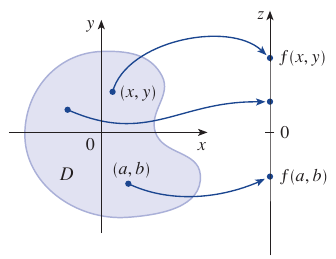
\includegraphics[width=\textwidth]{fvv1.png} 
    \end{minipage}
        
\begin{itemize}
    \item \textbf{Dominio ($D_f$):} Conjunto de pares $(x,y)$ para los cuales la función está definida. $D_f = \{ (x,y) \in \mathbb{R}^2 \mid \exists f(x,y) \}$.
    \item \textbf{Rango o Imagen ($R_f$):} Conjunto de valores $z$ que son imágenes de los pares en el dominio.
\end{itemize}

\textit{Ejemplo:} Para $f(x,y) = \ln(x^2 + y^2 - 4)$, el dominio es el conjunto de puntos tales que $x^2 + y^2 > 4$, es decir, el exterior de una circunferencia de radio 2 centrada en el origen.

\subsubsection{Gráfica}
    \noindent
    \begin{minipage}{0.55\textwidth}
        \begin{itemize}
            \item \textbf{Gráfica de la función (Curva):} Es el conjunto de puntos $(x,y,z)$ en $\mathbb{R}^3$ tal que $z = f(x,y)$.
            \item \textbf{Proyección de la gráfica (Superficie):} Es la proyección de la gráfica sobre el plano $xy$, que coincide con el dominio de la función.
        \end{itemize}    
    \end{minipage}
    \hfill 
    \begin{minipage}{0.40\textwidth}
            \centering
            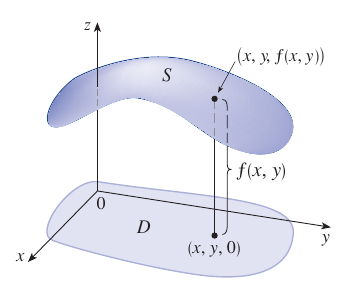
\includegraphics[width=\textwidth]{fvvgrafica.png} 
    \end{minipage}

\subsection{Curvas y Superficies de Nivel}
\begin{itemize}
    \noindent
    \begin{minipage}{0.55\textwidth}
            \item \textbf{Curva de Nivel:} Proyección sobre el plano $xy$ de la intersección de la superficie $z = f(x,y)$ con un plano horizontal $z = k$. Su ecuación es $f(x,y) = k$. \\ Muestra donde la gráfica de $f$ tiene altura $k$.
        \end{minipage}
    \hfill 
    \begin{minipage}{0.40\textwidth}
            \centering
            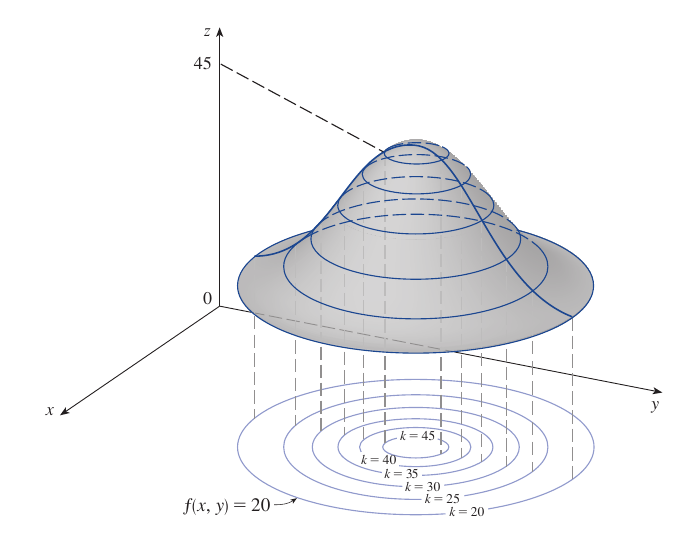
\includegraphics[width=\textwidth]{fvvcurvasdenivel.png} 
    \end{minipage}
    La superficie es pronunciada donde las curvas de nivel se juntan y más plana donde están separadas.

    \noindent
    \begin{minipage}{0.55\textwidth}
        \item \textbf{Superficie de Nivel:} Para funciones de tres variables $w = f(x,y,z)$, se obtienen haciendo $f(x,y,z) = k$. \\ 
            Si $(x,y,z)$ se mueve a lo largo de una superficie, el valor de $f$ permanece constante.
    \end{minipage}
    \hfill 
    \begin{minipage}{0.40\textwidth}
            \centering
            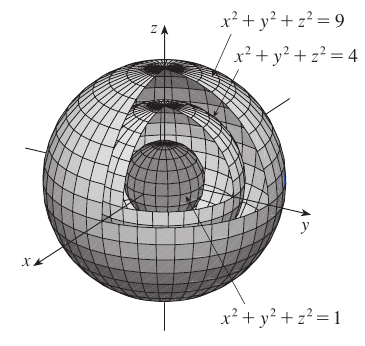
\includegraphics[width=\textwidth]{fvvsuperficeidenivel.png} 
    \end{minipage}
   
\end{itemize}

\newpage
\part{Límite y Continuidad}

\section{Límites en Funciones de Varias Variables}

\subsection{Definición Formal de Límite Doble}
Se dice que $L$ es el límite de $z = f(x,y)$ cuando $(x,y)$ tiende al punto $(a,b)$ si:
$$ \lim_{(x,y) \to (a,b)} f(x,y) = L \iff \forall \epsilon > 0, \exists \delta > 0 / \forall (x,y) \in D : $$ 
$$ 0 < \sqrt{(x-a)^2 + (y-b)^2} < \delta \implies |f(x,y) - L| < \epsilon $$

\begin{figure}[h]
    \centering
    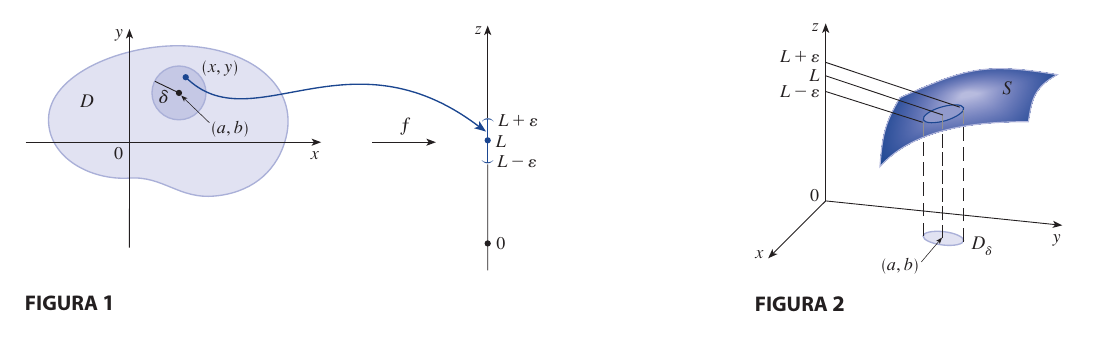
\includegraphics[width=1\textwidth]{fvvlimite.png}
    
    \vspace{0.5cm}
    
    % Columna para la Figura 1
    \begin{minipage}[t]{0.48\textwidth}
        \small
        \textbf{Figura 1:} Se muestra que si cualquier intervalo reducido $(L - \epsilon, L + \epsilon)$ se da alrededor de $L$, se puede determinar un disco $D_\delta$ con centro $(a,b)$ y radio $\delta > 0$ tal que $f$ mande todos los puntos de $D_\delta$ a puntos dentro del intervalo $(L - \epsilon, L + \epsilon)$.
    \end{minipage}
    \hfill % Espacio elástico entre columnas
    % Columna para la Figura 2
    \begin{minipage}[t]{0.48\textwidth}
        \small
        \textbf{Figura 2:} La superficie $S$ es la gráfica de $f$. Si $\epsilon > 0, \delta > 0 :$ si $(x,y)$ se encuentra dentro del disco $D_\delta$ y $(x,y) \neq (a,b) \Rightarrow S$ reside entre los planos $z = L - \epsilon$ y $z = L + \epsilon$.
    \end{minipage}
\end{figure}

 \noindent
    \begin{minipage}{0.55\textwidth}
        Para FVV $(x,y) \to (a,b)$ desde infinitas direcciones en cualquier trayectoria (mientras se mantenga dentro del dominio de $f$).
    \end{minipage}
    \hfill 
    \begin{minipage}{0.40\textwidth}
            \centering
            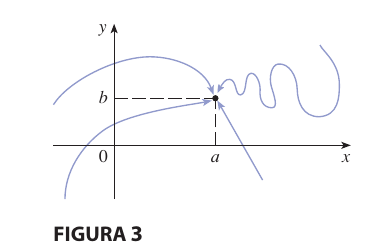
\includegraphics[width=\textwidth]{fvvlimite2.png} 
    \end{minipage}

\subsection{Límites Reiterados y Direccionales}
\begin{itemize}
    \item \textbf{Límites Reiterados (Sucesivos):} Se evalúa el límite aproximándose primero por una variable y luego por la otra. 
    $$ L_1 = \lim_{y \to b} \left[ \lim_{x \to a} f(x,y) \right] \quad ; \quad L_2 = \lim_{x \to a} \left[ \lim_{y \to b} f(x,y) \right] $$.
    Para que el límite doble exista, $L_1$ debe ser igual a $L_2$. Sin embargo, la igualdad de los reiterados \textbf{no garantiza} la existencia del límite doble.
    \item \textbf{Límites Direccionales:} Se evalúa el límite a lo largo de rectas ($y = mx$) o curvas ($y = cx^2$) que pasen por $(a,b)$. Si el límite depende de la dirección (ej. depende de $m$), entonces el límite doble no existe.
\end{itemize}

\section{Infinitésimos}
Una función $\alpha(x,y)$ es un infinitésimo para $(x,y) \to (x_0,y_0)$ si $\lim_{(x,y) \to (x_0,y_0)} \alpha(x,y) = 0$.
\textbf{Propiedades:}
\begin{enumerate}
    \item Suma o producto de infinitésimos es un infinitésimo.
    \item Infinitésimo por función acotada = Infinitésimo.
\end{enumerate}

\section{Continuidad}
Una función $z = f(x,y)$ es continua en $P_0(x_0,y_0)$ si cumple:
\begin{enumerate}
    \item $\exists f(x_0,y_0)$
    \item $\exists \lim_{(x,y) \to (x_0,y_0)} f(x,y) = L$
    \item $L = f(x_0,y_0)$
\end{enumerate}

Equivalentemente: $\lim_{(x,y) \to (x_0,y_0)} \Delta z = 0$.

\begin{tcolorbox}[title=Clasificación de Discontinuidades,colback=blue!5!white,colframe=blue!75!black]
    \begin{itemize}
        \item \textbf{Evitable:} Existe el límite doble, pero es distinto a $f(x_0,y_0)$ o la función no está definida en el punto.
        \item \textbf{Inevitable o Esencial:} El límite doble no existe.
    \end{itemize}
\end{tcolorbox}

\newpage
\part{Derivabilidad y Diferenciabilidad}

\section{Derivadas Parciales}
\subsection{Definición y Notación}
La derivada parcial de $f$ respecto a $x$ en el punto $(x_0,y_0)$ es:
$$ f_x(x_0,y_0) = \frac{\partial z}{\partial x} = \lim_{\Delta x \to 0} \frac{f(x_0+\Delta x, y_0) - f(x_0, y_0)}{\Delta x} $$
Análogamente para $y$ (con $\Delta y \to 0$).

\subsection{Interpretación Geométrica}
\begin{itemize}
    \item $\frac{\partial z}{\partial x}\Big|_{P_0}$: Es la pendiente de la recta tangente a la curva de intersección de la superficie $z = f(x,y)$ con el plano constante $y = y_0$.
    \item $\frac{\partial z}{\partial y}\Big|_{P_0}$: Es la pendiente de la recta tangente a la curva de intersección con el plano $x = x_0$.
\end{itemize}
Ambas tangentes determinan el \textbf{plano tangente} a la superficie.

\section{Diferenciabilidad}
\subsection{Incremento Total y Teorema del Valor Medio}
El incremento total está dado por: $\Delta z = f(x_0+\Delta x, y_0+\Delta y) - f(x_0,y_0)$.

\begin{tcolorbox}[title=Teorema del Valor Medio,colback=blue!5!white,colframe=blue!75!black]
    Si $f(x,y)$ tiene derivadas parciales continuas en una región, entonces el incremento total puede expresarse como:
    $$ \Delta z = f_x(x_0+\theta_1\Delta x, y_0)\Delta x + f_y(x_0, y_0+\theta_2\Delta y)\Delta y \quad \text{con } 0 < \theta_1, \theta_2 < 1 $$
\end{tcolorbox}

\subsection{Diferencial Total}
Una función es diferenciable en $(x_0,y_0)$ si su incremento total puede expresarse como:
$$ \Delta z = f_x(x_0,y_0)\Delta x + f_y(x_0,y_0)\Delta y + \alpha\Delta x + \beta\Delta y $$
donde $\alpha \to 0$ y $\beta \to 0$ cuando $(\Delta x, \Delta y) \to (0,0)$.

El \textbf{Diferencial Total} de la función es la parte lineal del incremento:
$$ dz = \frac{\partial f}{\partial x} dx + \frac{\partial f}{\partial y} dy $$

Geométricamente, $dz$ representa el incremento sobre el plano tangente, mientras que $\Delta z$ es el incremento sobre la superficie.

\subsection{Relación Continuidad-Derivabilidad-Diferenciabilidad}
\begin{itemize}
    \item Si $f$ es diferenciable $\implies f$ es continua.
    \item Si $f$ es diferenciable $\implies f$ es derivable.
    \item La derivabilidad no asegura continuidad, ni diferenciabilidad.
    \item \textbf{Condición Suficiente:} Si $f(x,y)$ es continua y sus derivadas parciales primeras son continuas en un entorno de $P_0$, entonces $f$ es diferenciable en $P_0$.
\end{itemize}

\section{Regla de la Cadena y Derivación Implícita}

\subsection{Regla de la Cadena}
Si $z = f(x,y)$ es diferenciable, y $x = g(u,v)$, $y = h(u,v)$:
$$ \frac{\partial z}{\partial u} = \frac{\partial z}{\partial x}\frac{\partial x}{\partial u} + \frac{\partial z}{\partial y}\frac{\partial y}{\partial u} $$
(Se aplica de forma análoga para $\frac{\partial z}{\partial v}$).

\subsection{Derivación Implícita}
Si una ecuación $F(x,y,z) = 0$ define implícitamente a $z = f(x,y)$, entonces:
$$ \frac{\partial z}{\partial x} = -\frac{F_x}{F_z} \quad \text{y} \quad \frac{\partial z}{\partial y} = -\frac{F_y}{F_z} \quad (F_z \neq 0) $$

\section{Derivada Direccional y Gradiente}

\subsection{Derivada Direccional}
Mide la variación instantánea de $z = f(x,y)$ en la dirección de un vector unitario $\vec{u} = \cos\theta \hat{i} + \sin\theta \hat{j}$. Se calcula como:
$$ D_{\vec{u}}f(x_0,y_0) = f_x(x_0,y_0)\cos\theta + f_y(x_0,y_0)\sin\theta $$

\subsection{Vector Gradiente}
Se define como $\nabla f(x,y) = f_x \hat{i} + f_y \hat{j}$.
\textbf{Propiedades:}
\begin{itemize}
    \item El gradiente es siempre perpendicular a la curva o superficie de nivel que pasa por el punto.
    \item $D_{\vec{u}}f(x,y) = \nabla f \cdot \vec{u}$.
    \item El valor máximo de la derivada direccional es $|\nabla f|$ y ocurre en la dirección del gradiente ($\cos\phi = 1$).
\end{itemize}

\section{Derivadas de Orden Superior}

\begin{tcolorbox}[title=Teorema de Schwarz (Conmutabilidad),colback=blue!5!white,colframe=blue!75!black]
    Si $z = f(x,y)$ tiene derivadas parciales mixtas $f_{xy}$ y $f_{yx}$ definidas y continuas en un entorno de $P_0(x_0,y_0)$, entonces son iguales:
    $$ f_{xy}(x_0,y_0) = f_{yx}(x_0,y_0) $$
\end{tcolorbox}

\newpage
\part{Aproximación y Optimización}

\section{Fórmula de Taylor}
Permite aproximar el valor de la función en un punto $(a+h, b+k)$ mediante un polinomio:
$$ f(x,y) = f(a,b) + f_x(a,b)(x-a) + f_y(a,b)(y-b) + $$
$$ \frac{1}{2!} \left[ f_{xx}(a,b)(x-a)^2 + 2f_{xy}(a,b)(x-a)(y-b) + f_{yy}(a,b)(y-b)^2 \right] + R_n $$

\section{Extremos Relativos}

\subsection{Condición Necesaria (Puntos Críticos)}
Si $f(x,y)$ tiene un extremo local en $(a,b)$ y sus derivadas parciales de primer orden existen en ese punto, entonces $(a,b)$ es un \textbf{punto crítico} tal que:
$$ f_x(a,b) = 0 \quad \text{y} \quad f_y(a,b) = 0 $$

\subsection{Condición Suficiente (Criterio del Hessiano)}
Sea $(a,b)$ un punto crítico. Se define el discriminante o Hessiano $H(x,y)$ como:
$$ H(a,b) = f_{xx}(a,b) \cdot f_{yy}(a,b) - [f_{xy}(a,b)]^2 $$

Se evalúa en el punto crítico $(a,b)$:
\begin{itemize}
    \item Si $H(a,b) > 0$ y $f_{xx}(a,b) > 0 \implies$ Hay un \textbf{Mínimo Relativo} en $(a,b)$.
    \item Si $H(a,b) > 0$ y $f_{xx}(a,b) < 0 \implies$ Hay un \textbf{Máximo Relativo} en $(a,b)$.
    \item Si $H(a,b) < 0 \implies$ No hay extremo, es un \textbf{Punto de Silla}.
    \item Si $H(a,b) = 0 \implies$ El criterio no es concluyente.
\end{itemize}

\end{document}